\documentclass[conference]{IEEEtran}
\IEEEoverridecommandlockouts
% The preceding line is only needed to identify funding in the first footnote. If that is unneeded, please comment it out.
\usepackage{cite}
\usepackage{amsmath,amssymb,amsfonts}
\usepackage{algorithmic}
\usepackage{graphicx}
\usepackage{textcomp}
\usepackage{xcolor}
\def\BibTeX{{\rm B\kern-.05em{\sc i\kern-.025em b}\kern-.08em
    T\kern-.1667em\lower.7ex\hbox{E}\kern-.125emX}}
\begin{document}

\title{Documentation of Lab work for group 8\\
}

\author{\IEEEauthorblockN{Wiktor Kochanek}
\IEEEauthorblockA{\textit{Electronic Engineering} \\
\textit{Hochschule Hamm-Lippstadt}\\
Lippstadt, Germany \\
wiktor.kochanek@stud.hshl.de}
\and
\IEEEauthorblockN{2\textsuperscript{nd} Given Name Surname}
\IEEEauthorblockA{\textit{dept. name of organization (of Aff.)} \\
\textit{name of organization (of Aff.)}\\
City, Country \\
email address or ORCID}
\and
\IEEEauthorblockN{3\textsuperscript{rd} Given Name Surname}
\IEEEauthorblockA{\textit{dept. name of organization (of Aff.)} \\
\textit{name of organization (of Aff.)}\\
City, Country \\
email address or ORCID}
\and
\IEEEauthorblockN{4\textsuperscript{th} Given Name Surname}
\IEEEauthorblockA{\textit{dept. name of organization (of Aff.)} \\
\textit{name of organization (of Aff.)}\\
City, Country \\
email address or ORCID}

}

\maketitle

\begin{abstract}
This document is a record of our group first forray into the world of autonomous driving.
\end{abstract}

\section{Introduction}
Motivated by a class assignement our group was tasked with creating a self-driving vehicle.
We achieved this by using line tracking sensors and ultrasonic sensors, but also attempted to implement a camera
and video streaming as the next step.

\section{Analyzing the specifications}

Our assignment came with clearly defined specifications:
\begin{itemize}
\item Line tracking system
\item Ultrasonic sensor integration
\item Camera streaming system
\end{itemize}
We split these objectives into two sections: car focused - line tracking and ultrasonic sensors systems - and camera focused - the streaming.
We then split the tasks inside our group so that each member can focus on a specific objective to bring the best possible results.


\section{Car focused specifications}
\subsection{Line tracking system}
The car was supposed to be able to follow a line around a track using two line tracking sensors. The specific implementation of such function was left to our own choice.
We decided to make a system that would allow the car to drive when it doesnt detect a line and react when it does detect a line.

\subsection{Ultrasonic sensors system}
The car was supposed to integrate a system using three ultrasonic sensors - what said system would influence was left to us to decide.
we settled on an obstacle avoiding system that would co-operate with the line tracking system - if there was an obstacle on the track the car
would attempt to drive around the obstacle and drive back onto the track.

\section{Camera focused specification}
The car was supposed to integrate a camera and a system that would allow it to stream the camera view onto an external computer.
for this task we used a Raspberri Pi with a camera module and a Mac computer.

\section{System Design}
The car will operate within 4 states for line tracking system and a pseudostate for the ultrasonic sensors sytem. Different enviromental inputs will influence the behaviour of the car.
\begin{figure}[h!]
	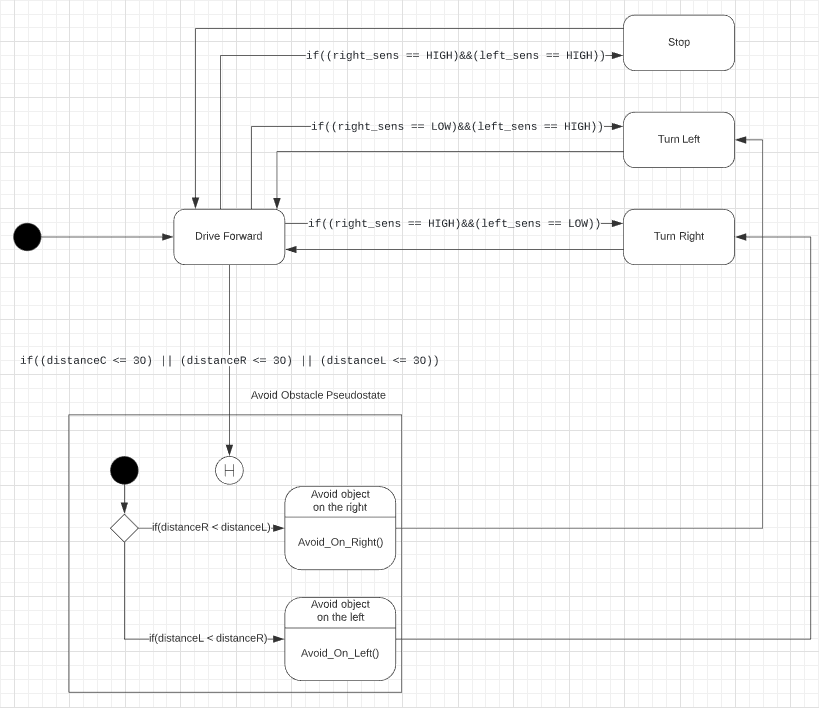
\includegraphics[width=\linewidth]{UMLStateDiagram.png}
	\caption{UML State Diagram}
	\label{fig:UMLSM1}
\end{figure}

The car will always begin in the line tracking state attempting to go forward. When one of the line tracking sensors detects that it has gone onto the line it will steer the car to get the sensor back off the line - Turn Right and Turn Left states. If it happens that both sensors are on the line at the same time the car will stop. Should the cars ultrasonic sensors detect an obstacle it will enter into the Avoiding Obstacles Pseudostate. It will then decide if the obstacle is closer to its right or left side and will attempt to avoid the obstacle on the other side. When it succesfully returns to the track the line tracking sensors will exit the car from the pseudostate and will reutrn line tracking functionality.

\section{Implementation of the system}
\subsection{Line tracking system}
The line tracking system was the first thing tackled in the car functionality. The first implementation was a simple use of "if" and "if else" functions - depending on which line tracking sensor was tirggered, speeds of motors would change to make the car drive forward, turn the correct way or stop completely. Later implementation made use of interrupts, which changed the motor speed in the interrupt service routine.
\begin{figure}[h!]
	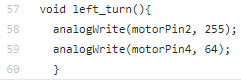
\includegraphics[width=\linewidth]{examplecode1.png}
	\caption{used interrupt service routine$^{1}$}
	\label{fig:EXC1}
\end{figure}
\footnote{lines of code in Fig. 2 do not represent actual content in the final source code}
Wile the interrupt solution was a great way to make the source code easy to understand and and the car ran very smoothly, it was scrapped during integration with ultrasonic sensor code as there were compatiblity problem. As such we settled on a "if" and "if else" functions solution.
\subsection{Obstacle avoidance system}
Implementation of the ultrasonic sensors was not specifically defined in the project requriements. Our design used them in a way to detect and obstacle in the way and attempt to drive around it. First the car had to know that there was an obstacle in front of it. This was achieved simply using an "if" function - if any of the three sensors detect an obstacle within 30cm of the car they will trigger the if condition and enter the car in the pseudostate of "avoid obstacle".
\begin{figure}[h!]
	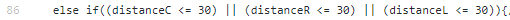
\includegraphics[width=\linewidth]{examplecode2.png}
	\caption{if condition detecting the obstacle}
	\label{fig:EXC2}
\end{figure}
After the car enter this pseudostate we have to choose which way is best to avoid the obstacle on - meaning that if theres a wall on our right, we want to turn to the left to clear it and vice versa. This is simply done by comparing the distance values on the right and left ultrasonic sensors - distanceR and distanceL respecitvelly. In this case we don't care about the centre distance as it doesnt influence our choice of side to avoid on. After the choice is made the car enters a loop that lets it go around an obstacle - in this example we will be avoiding an obstacle on the right (distanceL $<$ distanceR).
\begin{figure}[h!]
	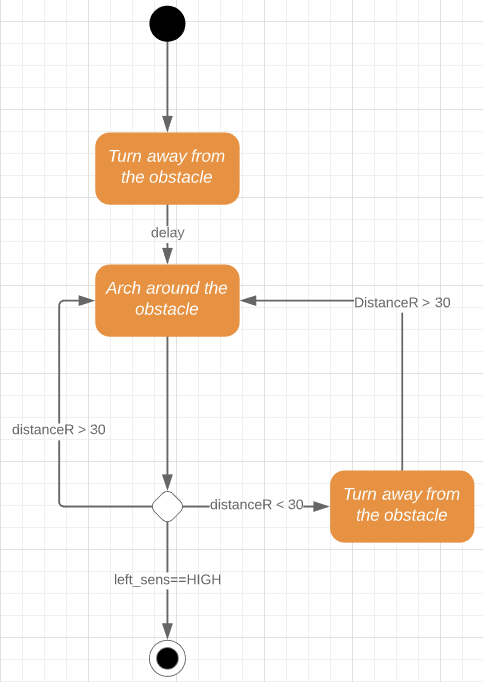
\includegraphics[width=\linewidth]{AvoidActivityDiagram.png}
	\caption{Activity diagram of the avoiding algorithm}
	\label{fig:AAD}
\end{figure}
After starting the avoiding algorithm the car will slowly arch around its obstacle. it is possible that the obstacle is longer than the arch diameter, so the car is able to detect obstacles in this mode and turn away again if needed.
This algorithm was designed to allow the car to leave its line in order to avoid the obstacle and detect when it is supposed to once again follow said line. In order to do that we had to have the car ignore one of the line tracking sensors for the duration of avoiding algorithm - in this case the right line tracking sensor - and then respect the sensor again when it gets back on the line. This was simply done by running the algorithm in a subfunction and including a simple if condition in the loop. The car arching around the obstacle is implemented using a while loop that relies on a variable set after the car decides on which side is the obstacle. The only way to stop that while loop is the active line tracking sensor - in this case the left one - to cross onto the line. The sensor triggering ends the while loop and the avoidance algorithm returning the car to its line tracking functionality.

\end{document}
